\documentclass{beamer}
\usetheme{Boadilla}
\usepackage{hyperref}
\usepackage{graphicx}
\usepackage{fancyvrb}
\usepackage{multicol}
\usepackage{subfig}
\usepackage[
    backend=biber, 
    natbib=true,
    style=numeric,
    sorting=none,
    style=verbose-ibid,
]{biblatex}
\addbibresource{citations.bib}
\usepackage{pgfpages}
\usepackage{xcolor}
\definecolor{ao(english)}{rgb}{0.0, 0.5, 0.0}
\definecolor{burgundy}{rgb}{0.5, 0.0, 0.13}
%\setbeameroption{show notes}
\setbeameroption{show notes on second screen=right}
%\setbeameroption{hide notes}

\title{Gabor's 1946 Theory of Communication}
\author{Sevag Hanssian}
\institute{MUMT 622, Winter 2021}
\setbeamertemplate{navigation symbols}{}

\begin{document}

\begin{frame}
\maketitle
\end{frame}

\begin{frame}
	\frametitle{Significance}
	Outcomes of Gabor's 1946 paper, ``Theory of Communication''\footfullcite{gabor1946}:
	\vspace{0.5em}
	\begin{enumerate}
		\item
			First introduction of the time-frequency uncertainty principle, leading to interest in wavelets\footfullcite{homage1}
		\item
			First use of the STFT for analysis of speech\footfullcite{textbook1}
			\begin{quote}
			The earliest application of a local Fourier analysis was by Dennis Gabor to the analysis of speech
			\end{quote}
		\item
			\vspace{-0.35em}
			Signal representation with Gabor elementary functions (Gaussian-modulated sinusoids) to minimize time-frequency uncertainty
	\end{enumerate}
\end{frame}

\begin{frame}
	\frametitle{Time-frequency resolution in the STFT}
	\begin{figure}
		\centering
		\subfloat[Good time resolution, poor frequency resolution]{{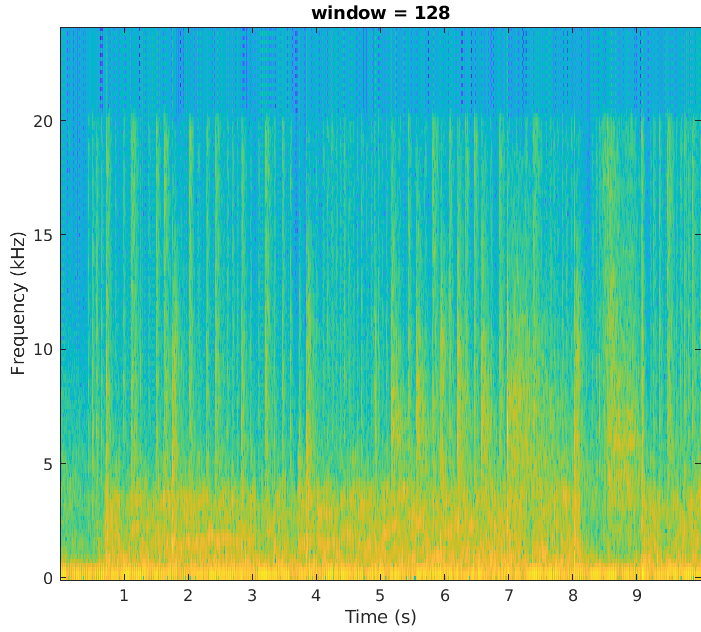
\includegraphics[width=6cm]{./stft_small.png} }}
		\subfloat[Good frequency resolution, poor time resolution]{{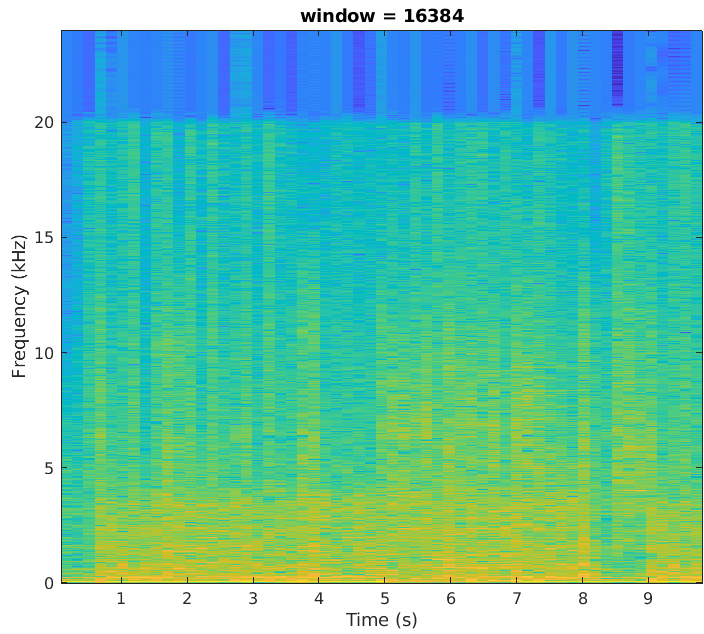
\includegraphics[width=6cm]{./stft_big.png} }}
		\caption{STFT, small vs. big window}
	\end{figure}
\end{frame}

\begin{frame}
	\frametitle{Time-frequency resolution in the STFT}
	\begin{figure}
		\centering
		\subfloat[Good time resolution, poor frequency resolution]{{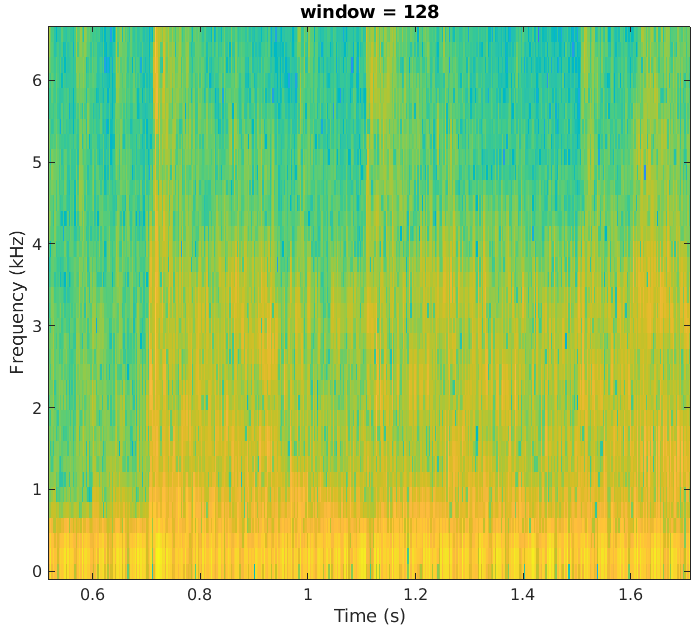
\includegraphics[width=6cm]{./stft_small_zoomed.png} }}
		\subfloat[Good frequency resolution, poor time resolution]{{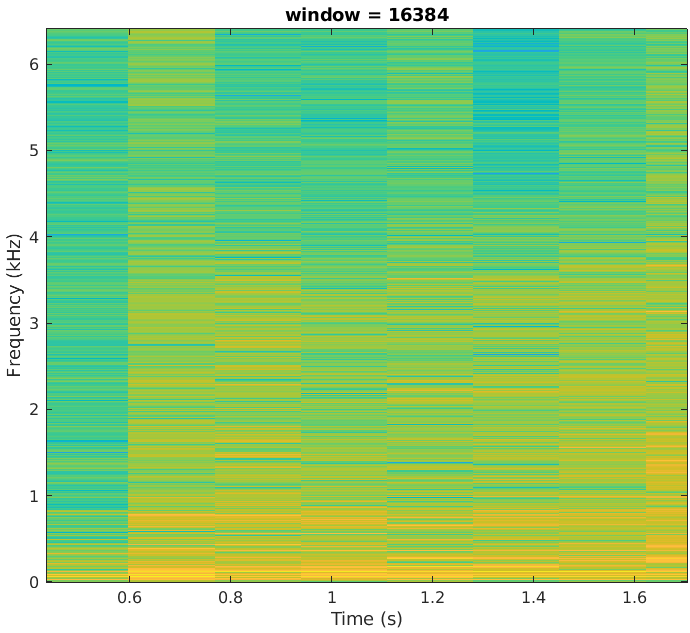
\includegraphics[width=6cm]{./stft_big_zoomed.png} }}
		\caption{STFT, small vs. big window}
	\end{figure}
\end{frame}

\begin{frame}
	\frametitle{Time-frequency trade-off -- intuition}
	\begin{figure}
		\centering
		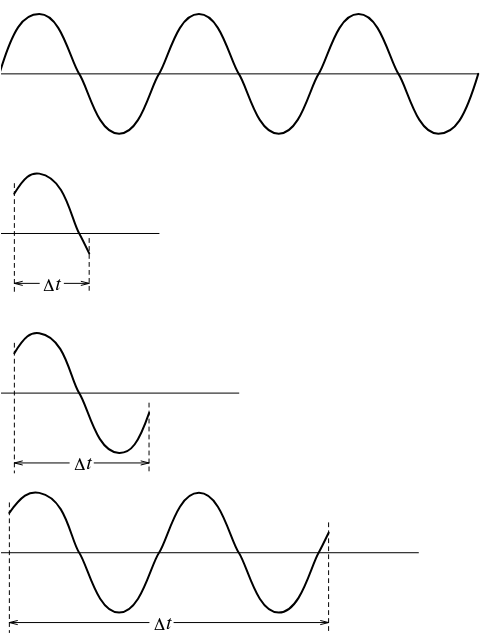
\includegraphics[height=5.5cm]{./gabor2.png}
		\caption{Improved frequency measurement over longer time intervals. The uncertainty in the frequency $\Delta f$ decreases as the measurement interval $\Delta t$ increases and vice versa\footfullcite{gabor2}}
	\end{figure}
\end{frame}

\begin{frame}
	\frametitle{Time-frequency tradeoff}
	Property of the Fourier transform
	\begin{figure}
		\centering
		\subfloat[Unit impulse vs. infinite sine wave\footfullcite{gabor1946}]{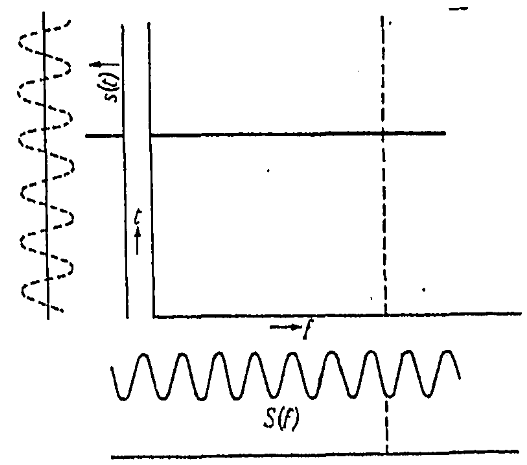
\includegraphics[width=4cm]{./gabor1.png}}
		\hspace{0.2em}
		\subfloat[Spread of a signal and its Fourier transform are inversely proportional\footfullcite{gabor2}]{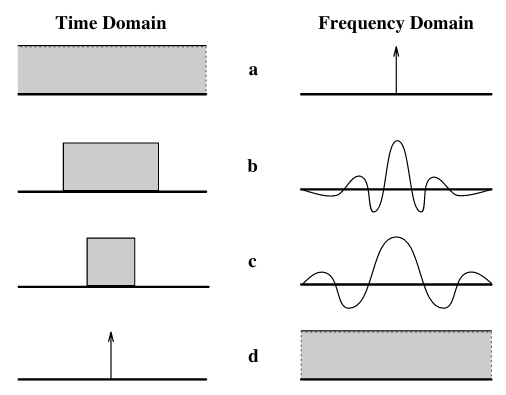
\includegraphics[width=5cm]{./gabor3.png}}
		\caption{Time vs. frequency}
	\end{figure}
\end{frame}

\begin{frame}
	\frametitle{Gabor's Uncertainty Principle}
\end{frame}

\begin{frame}
	\frametitle{Gabor's Uncertainty Principle, visual}
	\begin{figure}
		\centering
		\subfloat{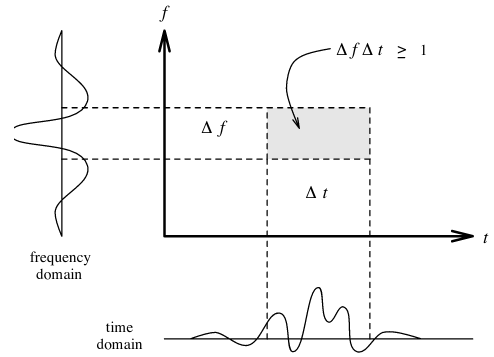
\includegraphics[height=4cm]{./tf-resolution2.png}}
		\hspace{0.35em}
		\subfloat{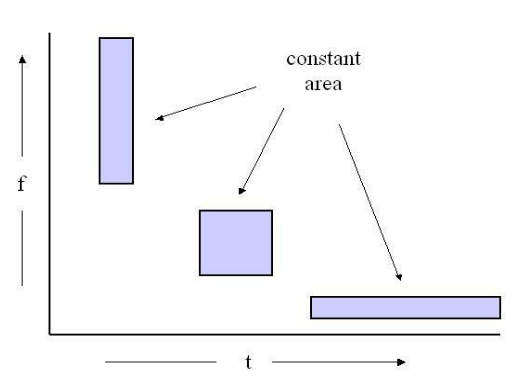
\includegraphics[height=4cm]{./tf-resolution.png}}
		\caption{The most a signal can be localized in the Fourier domain is into rectangles of size $\Delta t\Delta f = 1$}
	\end{figure}
\end{frame}

\end{document}
